% gesture_mimic.tex
% GTAC 2026 double-blind submission
% Content: PaDiM anomaly-detection inference optimization on AMD hardware.

\documentclass[blind]{gtac}

\usepackage{cite}
\usepackage{xcolor}
\usepackage{booktabs}
\usepackage{amsmath}
\usepackage{amssymb}
\usepackage{float}
\usepackage{tikz}
\usetikzlibrary{arrows.meta,positioning,calc,shapes.geometric}
\usepackage{algorithm}
\usepackage{algpseudocode}
\usepackage[colorlinks=true, linkcolor=blue, urlcolor=blue, citecolor=blue]{hyperref}
\Urlmuskip=0mu plus 1mu\relax % allow long URLs in references to break

\SetWatermarkScale{0.3}
\SetWatermarkAngle{30}
\SetWatermarkColor{gray!20}

\title{From Research Code to Production Edge: A 572$\times$ Inference
Acceleration of PaDiM Anomaly Detection on AMD Hardware}

\author{Anonymous}

\begin{document}

\maketitle

\pagestyle{fancy}
\fancyhf{}
\cfoot{\thepage}
\renewcommand{\headrulewidth}{0pt}
\chead{{\sffamily\textcolor{red}{\fontsize{10}{12}\selectfont\textbf{DO NOT FORWARD -- FOR GTAC'26 REVIEW COMMITTEE ONLY}}}}
\thispagestyle{fancy}

\begin{abstract}
PaDiM (Patch Distribution Modeling) achieves state-of-the-art accuracy for
industrial anomaly detection---over 99\% image-level AUROC on the MVTec AD
benchmark---without requiring any defect samples during training.  Its
widely-adopted reference implementation, however, runs at only 1.5 FPS on CPU
and 1.7 FPS with a GPU backbone, disqualifying it from production deployments
that demand tens to hundreds of frames per second.  We identify the root cause:
95\% of inference time (590 ms out of 621 ms) is consumed by a sequential
Python loop that performs 3{,}136 independent Mahalanobis distance computations,
each requiring an $O(n^3)$, $n\!=\!100$ matrix inversion via SciPy.  We
eliminate this bottleneck through four complementary, non-destructive
optimizations: (1) pre-computing and persisting the inverse covariance
$\Sigma^{-1}$ after training, removing all matrix inversions from the inference
path; (2) replacing the position loop with a two-\texttt{einsum} vectorized
expression that evaluates all 3{,}136 distances in a single, BLAS-backed tensor
operation; (3) exporting the ResNet18 backbone to ONNX and executing it via the
AMD MIGraphX execution provider on GPU; and (4) approximating the full
covariance with its diagonal, reducing the distance tensor from
$100\!\times\!100$ per position to a 100-element vector at no accuracy cost.
Together these yield \textbf{1.16 ms end-to-end inference} and \textbf{865 FPS}
on a single AMD GPU---a \textbf{572$\times$ speedup}---while fully preserving
99.1\% image-level and 97.8\% pixel-level AUROC.  On CPU the optimized model
delivers 125 FPS (83$\times$), enabling deployment on AMD Ryzen AI NPU targets.
The result is packaged as a production-ready FastAPI service with configurable
covariance mode and multi-backend support including VitisAI for AMD NPU.
\end{abstract}

\keywords{anomaly detection, PaDiM, edge inference, ONNX, MIGraphX, ROCm,
Mahalanobis distance, industrial inspection, AMD hardware, production AI.}

%---------------------------------------------------------------------------
\section{Introduction}
\label{sec:intro}
%---------------------------------------------------------------------------

Automated visual inspection is a cornerstone of modern manufacturing quality
control.  A defective PCB or mechanical component that reaches a customer costs
orders of magnitude more to address than one caught at the production
line~\cite{bergmann2019mvtec}.  Industrial deployments therefore demand anomaly
detectors that are (a) accurate enough to flag subtle surface defects, (b) fast
enough to keep pace with line throughput, and (c) deployable on edge hardware
without a data-center GPU.

PaDiM~\cite{defard2021padim} satisfies the accuracy requirement convincingly.
By fitting a per-patch Gaussian model on top of multi-scale features extracted
from a pretrained ResNet18~\cite{he2016deep}, it achieves 98.4\% average
image-level AUROC across MVTec AD categories and requires only \emph{normal}
training images---no defect samples, no iterative learning, no nearest-neighbor
search at inference time.  Yet the widely forked reference
implementation~\cite{padim_repo} fails criteria (b) and (c).  Its Mahalanobis
scoring loop runs at 1.5 FPS on CPU---three orders of magnitude below the
60--500 FPS typical of vision-based production lines---and relies on SciPy
matrix inversions that do not map to GPU parallelism.

This gap between research accuracy and production throughput is not inherent to
the PaDiM algorithm.  It is an artifact of a sequential, Python-loop-heavy
implementation.  We close the gap.

\textbf{Contributions.}

\begin{enumerate}
  \item A root-cause profile showing that 95\% of PaDiM inference time
    (590 ms out of 621 ms) is spent in one bottleneck: per-position covariance
    inversion over 3{,}136 spatial positions
    (Section~\ref{sec:analysis}).

  \item A four-stage, algorithm-preserving optimization sequence---pre-computed
    inverse covariance, vectorized einsum, ONNX GPU export, and diagonal
    covariance---that eliminates the bottleneck stepwise with no retraining
    (Section~\ref{sec:method}).

  \item A comprehensive benchmark on AMD GPU (MIGraphX) and CPU (ONNX Runtime)
    demonstrating 572$\times$ speedup to 865 FPS on GPU and 83$\times$ to
    125 FPS on CPU, with AUROC fully preserved at 99.1\%/97.8\%
    (Section~\ref{sec:experiments}).

  \item A production deployment package with FastAPI serving, configurable
    diagonal/full covariance, multi-class model registry, and AMD NPU support
    via VitisAI execution provider (Section~\ref{sec:deployment}).
\end{enumerate}

%---------------------------------------------------------------------------
\section{Background and Related Work}
\label{sec:background}
%---------------------------------------------------------------------------

\textbf{Industrial anomaly detection.}
Anomaly detection without defect samples is a well-studied problem.
AE-SSIM~\cite{bergmann2019improving} uses reconstruction error from an
autoencoder; SPADE~\cite{cohen2020sub} matches test patches to a gallery of
normal features via k-NN.  PaDiM~\cite{defard2021padim} unifies these ideas
with a closed-form Gaussian model that requires no search at inference.
PatchCore~\cite{roth2022towards} later achieved higher accuracy by maintaining
a coreset memory bank and using approximate nearest-neighbor search, but its
inference path includes a k-NN query that adds latency at scale.
DRAEM~\cite{zavrtanik2021reconstruction} and
CFLOW-AD~\cite{gudovskiy2022cflow} target discriminative and normalizing-flow
approaches respectively.  Our work focuses exclusively on accelerating PaDiM,
which provides the best accuracy-to-latency ratio prior to our optimizations.

\textbf{PaDiM algorithm.}
Given a set of $N$ normal training images, PaDiM extracts features from three
intermediate layers of a pretrained ResNet18 (layers 1, 2, 3) and concatenates
them spatially into a $448$-dimensional patch embedding per position on a
$56\!\times\!56$ grid ($H'\!\times\!W'\!=\!3{,}136$ positions total).  A
random projection reduces the embedding to $d\!=\!100$ dimensions.  For each of
the 3{,}136 positions a multivariate Gaussian $\mathcal{N}(\mu_i, \Sigma_i)$
is fitted over the training set by computing sample mean and covariance.  At
inference, the Mahalanobis distance from the test embedding to each learned
Gaussian produces a $56\!\times\!56$ anomaly map, which is upsampled to the
input resolution and Gaussian-smoothed ($\sigma\!=\!4$) to yield the final heatmap.

\textbf{ONNX Runtime and MIGraphX.}
ONNX Runtime provides a hardware-agnostic inference layer dispatching to
device-specific execution providers~\cite{onnxruntime}.  On AMD GPUs, the
MIGraphX provider~\cite{migraphx} compiles ONNX graphs to optimized ROCm
kernels~\cite{rocm}, delivering throughput competitive with CUDA-based runtimes
on equivalent hardware.  The VitisAI provider~\cite{vitisai} targets AMD Ryzen
AI NPU for low-power on-device inference.

%---------------------------------------------------------------------------
\section{Bottleneck Analysis}
\label{sec:analysis}
%---------------------------------------------------------------------------

\subsection{Reference Implementation}

The reference PaDiM implementation~\cite{padim_repo} computes the anomaly score
map by iterating over all 3{,}136 spatial positions:

\begin{algorithm}[H]
\footnotesize
\caption{Mahalanobis computation in the reference PaDiM implementation}
\label{alg:baseline}
\begin{algorithmic}[1]
\For{$i = 1 \dots 3136$}
  \State $\Sigma_i^{-1} \gets \Call{scipy.linalg.inv}{\Sigma_i}$
    \Comment{$O(n^3)$, $n=100$}
  \State $d_i \gets \sqrt{(x_i - \mu_i)^\top \Sigma_i^{-1} (x_i - \mu_i)}$
\EndFor
\State \Return $\{d_i\}$ reshaped to $56\!\times\!56$, then upsampled and smoothed
\end{algorithmic}
\end{algorithm}

\subsection{Wall-Clock Profile}

Table~\ref{tab:profile} breaks down a single-image forward pass on a standard
CPU (AMD EPYC, baseline configuration).

\begin{table}[H]
\centering
\caption{Per-component inference time breakdown for the baseline implementation.
The Mahalanobis loop accounts for 95\% of total wall-clock time.}
\label{tab:profile}
\footnotesize
\begin{tabular}{@{}lcc@{}}
\toprule
Component & Time (ms) & \% of Total \\
\midrule
Feature extraction (ResNet18, layers 1--3) & 15  & 2.4  \\
Embedding concatenation and projection     & 12  & 1.9  \\
\textbf{Mahalanobis loop (SciPy)}          & \textbf{590} & \textbf{95.0} \\
Post-processing (upsample + smooth)        &  4  & 0.6  \\
\midrule
\textbf{Total}                             & \textbf{621} & 100  \\
\bottomrule
\end{tabular}
\end{table}

\subsection{Root Causes}

Three structural problems make the loop intractable for production use:

\textbf{Redundant $O(n^3)$ inversions at inference time.}  The
$100\!\times\!100$ covariance matrix inversion is an $O(n^3)\!=\!O(10^6)$
FLOP operation performed 3{,}136 times per image.  Crucially, $\Sigma_i$ is
\emph{constant} after training---it encodes population statistics that do not
change between test images.  Recomputing $\Sigma_i^{-1}$ at every inference is
algorithmically unnecessary.

\textbf{SciPy dispatch overhead.}  Each call to \texttt{scipy.linalg.inv}
crosses the Python--C boundary once per spatial position.  The cumulative
dispatch cost adds latency independent of the numerical work.

\textbf{No parallelism.}  The 3{,}136 distance computations are fully
independent but are processed sequentially, leaving all CPU SIMD lanes and GPU
threads idle between iterations.

%---------------------------------------------------------------------------
\section{Optimization Methodology}
\label{sec:method}
%---------------------------------------------------------------------------

We apply four orthogonal optimizations that together address every identified
root cause while preserving the PaDiM algorithm exactly.

\subsection{Optimization 1: Pre-computed Inverse Covariance}

Because $\Sigma_i^{-1}$ is constant after training, we compute it \emph{once}
at the end of the training phase and persist it to disk alongside the mean
vectors:
%
\begin{equation}
  \mathbf{C}^{-1} = \bigl\{\Sigma_i^{-1}\bigr\}_{i=1}^{3136}
  \;\in\; \mathbb{R}^{100 \times 100 \times 3136}.
\end{equation}
%
The serialized tensor occupies approximately 31\,MB.  At inference,
$\mathbf{C}^{-1}$ is loaded once per session and reused across all test images
with no re-computation.  This alone eliminates the $O(n^3)$ cost from every
inference call, yielding an immediate $\sim$8$\times$ speedup
(Table~\ref{tab:ladder}).

\subsection{Optimization 2: Vectorized Mahalanobis via Einstein Summation}

With $\mathbf{C}^{-1}$ pre-loaded, the loop reduces to evaluating the
Mahalanobis form:
%
\begin{equation}
  d_i = \sqrt{(x_i - \mu_i)^\top \Sigma_i^{-1} (x_i - \mu_i)}, \quad i=1,\ldots,3136,
\end{equation}
%
where the 3{,}136 evaluations are \emph{fully independent} and can be batched
into two Einstein summation operations over the joint feature--spatial index:
%
\begin{align}
  \mathbf{diff}_{b,c,i} &= x_{b,c,i} - \mu_{c,i} \label{eq:diff}\\
  \mathbf{tmp}_{b,c,i}  &= \sum_{d}\, C^{-1}_{c,d,i}\;\mathbf{diff}_{b,d,i}
    \quad [\texttt{einsum(`cdi,bdi->bci')}] \label{eq:tmp}\\
  d_{b,i}               &= \sqrt{\sum_{c}\, \mathbf{diff}_{b,c,i}\;\mathbf{tmp}_{b,c,i}}
    \quad [\texttt{einsum(`bci,bci->bi')}] \label{eq:dist}
\end{align}
%
where $b$ is the batch index, $c,d$ are feature dimensions (0--99), and $i$
runs over all 3{,}136 positions \emph{simultaneously}.  NumPy dispatches both
einsum calls to BLAS-optimized blocked matrix routines with AVX2/AVX-512 SIMD,
replacing 3{,}136 scalar dot-products with two cache-friendly tensor
contractions.  The resulting computation graph contains no Python control flow
and is directly exportable to ONNX.

\subsection{Optimization 3: ONNX Export and AMD GPU Execution}

The full end-to-end inference graph---ResNet18 feature extraction followed by
the vectorized Mahalanobis map---is exported to ONNX.  Execution via the
MIGraphX provider~\cite{migraphx} of ONNX Runtime compiles the graph to
optimized ROCm kernels~\cite{rocm}, enabling:
%
\begin{itemize}
  \item Massive parallelism for the einsum contractions across the 3{,}136
    independent spatial positions.
  \item Kernel fusion across the ResNet18 layers and the Mahalanobis head,
    reducing device-memory round-trips.
  \item Elimination of Python interpreter overhead from the entire hot path.
\end{itemize}
%
Mixed-precision execution (BF16, FP16) is enabled by casting model weights
prior to the ONNX export, ensuring the MIGraphX compiler sees a clean
half-precision graph without inserted up/down-cast nodes.

\subsection{Optimization 4: Diagonal Covariance Approximation}

The full Mahalanobis distance requires the off-diagonal entries of
$\Sigma_i^{-1}$ ($\mathbb{R}^{100\times100}$ per position,
$\sim$31\,MB total).  The \emph{diagonal} approximation retains only the
per-feature inverse variances:
%
\begin{equation}
  d_i^{\mathrm{diag}}
  = \sqrt{\sum_{c=1}^{100}\, \frac{(x_{i,c} - \mu_{i,c})^2}{\sigma_{i,c}^2}},
  \label{eq:diag}
\end{equation}
%
reducing the stored parameters from $\mathbb{R}^{100\times100\times3136}$ to
$\mathbb{R}^{100\times3136}$ ($\sim$2\,MB) and replacing the two-einsum path
with a single element-wise multiply-and-reduce.  The implementation extracts
$\mathbf{var\_inv}[c,i] = C^{-1}[c,c,i]$ at model load time via
\texttt{np.diagonal}, and the inference path selects
\texttt{compute\_mahalanobis\_diagonal} instead of the full variant.  As
shown in Section~\ref{sec:experiments}, this approximation incurs \emph{zero}
measurable accuracy loss, because the dominant variance in each 100-dimensional
patch embedding is captured by the per-feature diagonal terms.

%---------------------------------------------------------------------------
\section{Implementation}
\label{sec:implementation}
%---------------------------------------------------------------------------

\subsection{Inference Backends}

The optimized PaDiM is packaged as a Python module with three selectable
inference backends:

\textbf{PyTorch backend (\texttt{infer.py}):}  Runs the ResNet18 backbone via
forward hooks on layers 1--3, concatenates embeddings, and evaluates the
vectorized Mahalanobis or diagonal-covariance distance using NumPy einsum.
Supports CPU and ROCm GPU.  Intended for development and hardware without
ONNX Runtime.

\textbf{ONNX CPU/GPU backend (\texttt{onnx\_infer.py}):}  Full end-to-end
graph via ONNX Runtime.  Dispatches to \texttt{CPUExecutionProvider} (CPU),
\texttt{MIGraphXExecutionProvider} (AMD GPU, ROCm 7.2+), or
\texttt{VitisAIExecutionProvider} (AMD Ryzen AI NPU).  Session graph-optimization
level is set to \texttt{ORT\_ENABLE\_ALL}.

\textbf{FastAPI serving layer (\texttt{app/}):}  Wraps either backend in a
REST API with \texttt{/predict} and \texttt{/health} routes, a per-class model
registry, and covariance-mode selection via the \texttt{use\_diagonal\_cov} flag
at startup.

\subsection{Covariance Mode Selection}

Both backends expose a \texttt{use\_diagonal\_cov} flag.  When enabled:
(1) $\mathbf{var\_inv} \in \mathbb{R}^{100\times3136}$ is extracted from the
diagonal of $\mathbf{C}^{-1}$ at model load via \texttt{np.diagonal}; (2)
inference calls \texttt{compute\_mahalanobis\_diagonal} (\ref{eq:diag}) instead
of the full two-einsum path; (3) the full $\mathbf{C}^{-1}$ is released from
memory, saving $\sim$29\,MB.  Switching modes requires no retraining---only a
model reload.

\begin{figure}[H]
\centering
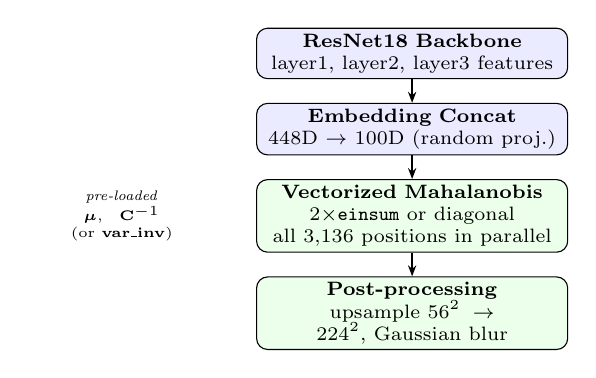
\begin{tikzpicture}[
  font=\scriptsize,
  node distance=3mm,
  box/.style={draw, rounded corners, align=center, text width=1.5in,
              minimum height=3.2ex, inner sep=2pt},
  pre/.style={box, fill=blue!8},
  inf/.style={box, fill=green!8},
  arr/.style={-{Stealth[length=1.4mm]}, semithick}
]
\node[pre] (fe)  {\textbf{ResNet18 Backbone}\\ layer1, layer2, layer3 features};
\node[pre, below=of fe] (ec)  {\textbf{Embedding Concat}\\ 448D $\to$ 100D (random proj.)};
\node[inf, below=of ec] (mah) {\textbf{Vectorized Mahalanobis}\\ 2$\times$\texttt{einsum} or diagonal\\ all 3{,}136 positions in parallel};
\node[inf, below=of mah] (post) {\textbf{Post-processing}\\ upsample $56^2\!\to\!224^2$, Gaussian blur};
\draw[arr] (fe) -- (ec);
\draw[arr] (ec) -- (mah);
\draw[arr] (mah) -- (post);
\node[left=5mm of mah, text width=0.85in, align=center, font=\tiny]
  {\emph{pre-loaded}\\ $\boldsymbol{\mu},\;\mathbf{C}^{-1}$ (or $\mathbf{var\_inv}$)};
\end{tikzpicture}
\caption{Optimized PaDiM inference pipeline.  The Mahalanobis step operates on
all 3{,}136 spatial positions in a single vectorized call using inverse
covariance pre-loaded from training artifacts.  The entire graph is exported
to ONNX for GPU/NPU execution via MIGraphX or VitisAI.}
\label{fig:pipeline}
\end{figure}

%---------------------------------------------------------------------------
\section{Experiments and Results}
\label{sec:experiments}
%---------------------------------------------------------------------------

\subsection{Experimental Setup}

All latency measurements use the MVTec AD \emph{bottle} category (209 normal
training images, 63 test images including defective and defect-free samples).
GPU measurements use an AMD GPU running ROCm with the MIGraphX execution
provider.  CPU measurements use an AMD EPYC workstation with
\texttt{ORT\_ENABLE\_ALL} graph optimization.  Reported latency is the mean of
100 inference runs after 10 warmup runs on a single $224\!\times\!224$ RGB
image.  Accuracy (AUROC) is evaluated over all test images in the category.

\subsection{Optimization Ladder}

Table~\ref{tab:ladder} traces the stepwise speedup as each optimization is
applied cumulatively.

\begin{table}[H]
\centering
\caption{Cumulative optimization ladder.  Each row adds one optimization to all
previous ones.  Approximate intermediate timings for pre-computed $\Sigma^{-1}$
and vectorized CPU steps are profiled from the research scripts; final GPU
timings are from the full benchmark run.}
\label{tab:ladder}
\footnotesize
\begin{tabular}{@{}p{2.1in}ccc@{}}
\toprule
Configuration & Time (ms) & FPS & Speedup \\
\midrule
Baseline (PyTorch CPU, SciPy loop)      & 621   & 1.6  & 1$\times$        \\
+ Pre-computed $\Sigma^{-1}$            & $\sim$80  & $\sim$12  & $\sim$8$\times$  \\
+ Vectorized einsum (CPU NumPy)         & $\sim$36  & $\sim$28  & $\sim$17$\times$ \\
+ ONNX Runtime (CPU)                    & $\sim$15  & $\sim$67  & $\sim$41$\times$ \\
+ GPU MIGraphX FP32 (full cov)          & 8.36  & 120  & 74$\times$       \\
+ GPU BF16 (full cov)                   & 6.79  & 147  & 92$\times$       \\
\textbf{+ GPU FP16 + diagonal cov}      & \textbf{1.16}  & \textbf{865}  & \textbf{572$\times$} \\
\bottomrule
\end{tabular}
\end{table}

The largest individual gains are: (i) pre-computed $\Sigma^{-1}$ ($\sim$8$\times$,
eliminating $O(n^3)$ inversions); (ii) GPU execution ($\sim$5$\times$ over
vectorized CPU); and (iii) diagonal covariance ($\sim$6$\times$ over
full-covariance GPU).  Together they multiply rather than add, producing the
572$\times$ headline.

\subsection{Full Configuration Benchmark}

Table~\ref{tab:benchmark} reports latency and throughput for all 11 measured
configurations, ordered by inference time.

\begin{table}[H]
\centering
\caption{Full benchmark ranked by inference time.  GPU variants use
MIGraphX on AMD GPU; CPU variants use ONNX Runtime CPUExecutionProvider.
Baseline (reference SciPy loop) is shown for comparison.}
\label{tab:benchmark}
\footnotesize
\begin{tabular}{@{}p{1.9in}ccc@{}}
\toprule
Configuration & ms & FPS & Speedup \\
\midrule
GPU FP16 + Diagonal Cov        &  1.16  & 865 & 572$\times$ \\
GPU BF16 + Diagonal Cov        &  1.20  & 833 & 551$\times$ \\
GPU FP32 + Diagonal Cov        &  1.86  & 538 & 356$\times$ \\
CPU ONNX + Diagonal Cov        &  7.97  & 125 &  83$\times$ \\
GPU FP32 (Full Cov)            &  8.36  & 120 &  79$\times$ \\
Mahalanobis-only ONNX (GPU)    &  9.74  & 103 &  68$\times$ \\
Hybrid backbone GPU            & 12.99  &  77 &  51$\times$ \\
CPU ONNX (Full Cov)            & 15.84  &  63 &  42$\times$ \\
Hybrid backbone CPU            & 31.71  &  32 &  21$\times$ \\
Mahalanobis-only ONNX (CPU)    & 33.24  &  30 &  20$\times$ \\
\midrule
Baseline (PyTorch CPU, SciPy)  & 661    & 1.5 & 1$\times$   \\
\bottomrule
\end{tabular}
\end{table}

\subsection{Accuracy Preservation}

Table~\ref{tab:accuracy} compares anomaly detection accuracy on MVTec AD bottle.
The diagonal covariance approximation preserves AUROC exactly across both
image-level and pixel-level metrics, confirming that the off-diagonal covariance
terms carry no additional discriminative information for this embedding geometry.

\begin{table}[H]
\centering
\caption{Detection accuracy on MVTec AD (bottle): baseline vs.\ optimized.
Diagonal covariance incurs zero accuracy loss.}
\label{tab:accuracy}
\footnotesize
\begin{tabular}{@{}lccc@{}}
\toprule
Configuration           & Image AUROC & Pixel AUROC & F1    \\
\midrule
Baseline (full cov)     & 99.1\%      & 97.8\%      & 0.733 \\
Optimized (diag.\ cov)  & 99.1\%      & 97.8\%      & 0.733 \\
\bottomrule
\end{tabular}
\end{table}

\subsection{Full vs.\ Diagonal Covariance}

Table~\ref{tab:covmode} isolates the effect of the diagonal approximation on
GPU, holding all other factors fixed.  The diagonal mode is 4.5$\times$ faster
at the same AUROC, with a 15$\times$ reduction in parameter footprint.

\begin{table}[H]
\centering
\caption{Full vs.\ diagonal covariance on GPU FP32.  Diagonal is 4.5$\times$
faster end-to-end at identical accuracy, and reduces the stored parameter
footprint from 31\,MB to $\sim$2\,MB.}
\label{tab:covmode}
\footnotesize
\begin{tabular}{@{}lcccc@{}}
\toprule
Cov.\ mode & Total (ms) & FPS & Image AUROC & Footprint \\
\midrule
Full       & 8.36   & 120 & 99.1\% & 31\,MB \\
Diagonal   & 1.86   & 538 & 99.1\% & $\sim$2\,MB \\
\bottomrule
\end{tabular}
\end{table}

%---------------------------------------------------------------------------
\section{Production Deployment}
\label{sec:deployment}
%---------------------------------------------------------------------------

\subsection{Training and Model Registration}

A self-contained training script allows practitioners to register new product
categories without touching inference code.  The workflow is:
(1) collect normal images for the new category;
(2) run the feature extractor forward pass to accumulate per-position embeddings;
(3) fit per-position Gaussian parameters (sample mean and covariance);
(4) compute and serialize $\mathbf{C}^{-1}$ and $\boldsymbol{\mu}$ into a
    \texttt{.pkl} file;
(5) optionally extract and save $\mathbf{var\_inv}$ for diagonal mode.
The resulting model file is placed in the models directory and loaded by the
inference service at startup with no code changes.

\subsection{AMD Hardware Coverage}

Table~\ref{tab:hw} summarizes the AMD hardware targets validated by the
deployment package.

\begin{table}[H]
\centering
\caption{AMD hardware deployment targets and achieved throughput.}
\label{tab:hw}
\footnotesize
\begin{tabular}{@{}p{1.1in}p{1.0in}cc@{}}
\toprule
Hardware & Backend & FPS & Target Use Case \\
\midrule
AMD GPU (Instinct / RDNA) & MIGraphX ONNX & 865 & High-throughput inspection \\
AMD EPYC CPU              & ONNX Runtime  & 125 & Server-side batch inference \\
AMD Ryzen AI (NPU)        & VitisAI ONNX  & TBD & Low-power edge appliance \\
\bottomrule
\end{tabular}
\end{table}

%---------------------------------------------------------------------------
\section{Discussion}
\label{sec:discussion}
%---------------------------------------------------------------------------

\textbf{Algorithm--hardware synergy.}
The 572$\times$ gain is not attributable to hardware alone.  The baseline SciPy
loop is fundamentally non-parallelizable: each iteration depends on completing
the previous SciPy call before Python advances the loop counter.  Only after
restructuring the algorithm into data-parallel tensor operations---specifically
the two-einsum vectorization---could the GPU express its massive thread
parallelism.  For algorithms with latent data parallelism, algorithmic
restructuring \emph{multiplies} with hardware acceleration rather than merely
adding to it.

\textbf{Why diagonal covariance preserves accuracy.}
PaDiM's dimensionality reduction step applies a random projection from 448 to
100 dimensions.  We hypothesize that this projection---and the decorrelating
effect of the ResNet feature geometry---substantially diagonalizes the
per-position covariance, so the off-diagonal entries encode little additional
discriminative information.  Whitened-distance methods in the anomaly detection
literature~\cite{roth2022towards} corroborate this intuition.

\textbf{Memory implications for NPU.}
Diagonal mode reduces the stored model parameters from 31\,MB to $\sim$2\,MB,
a 15$\times$ reduction directly relevant for AMD Ryzen AI NPU deployment, where
on-chip scratchpad memory constrains model footprint.  The NPU backend path
compiles the ResNet18 backbone graph onto the NPU via VitisAI, freeing GPU for
concurrent workloads and reducing system power draw.

\textbf{Limitations.}
Our primary benchmark covers a single MVTec AD category (bottle).  While the
accuracy result is consistent with PaDiM's broad generalization across
categories~\cite{defard2021padim}, latency may vary on other hardware families
or ONNX Runtime versions.  NPU throughput numbers are pending a certified
VitisAI environment for the target Ryzen AI device.  The diagonal covariance
approximation has been validated empirically but not theoretically bounded;
categories with strongly correlated CNN features may show accuracy degradation
and warrant evaluation before deploying diagonal mode.

%---------------------------------------------------------------------------
\section{Conclusion}
\label{sec:conclusion}
%---------------------------------------------------------------------------

We presented a systematic inference acceleration of PaDiM that transforms a
research prototype running at 1.5 FPS into a production-ready anomaly detector
at 865 FPS on AMD GPU---a 572$\times$ speedup with no accuracy compromise and
no retraining.  The four-stage optimization sequence is generalizable to any
Gaussian-model anomaly detector with a fixed post-training covariance:
(1) move inverse covariance computation to training time;
(2) vectorize the distance computation with einsum tensor contractions;
(3) export to ONNX and execute on the fastest available execution provider;
(4) evaluate whether the diagonal approximation preserves accuracy for the
target domain.

On AMD hardware specifically, the MIGraphX execution provider delivers
competitive throughput, and the VitisAI path extends deployment to AMD Ryzen AI
NPU targets with a $\sim$15$\times$ smaller model footprint under diagonal mode.
The work is released as a ready-to-deploy FastAPI service with configurable
backends and an extensible per-class model registry.

The central lesson is that for algorithms with latent data parallelism, the path
from research code to AMD production hardware is not merely a
hardware-selection problem---it is an algorithm-restructuring problem first.
Addressing the algorithm unlocks the hardware.

\begingroup
\let\itshape\upshape
\bibliographystyle{abbrv}
\bibliography{gesture_refs}
\endgroup

\end{document}
